\documentclass[11pt, a4paper]{article}

% --- Packages ---
\usepackage[margin=1in]{geometry} % 1-inch margins
\usepackage{amsmath, amssymb}   % Essential math symbols and tools
\usepackage{graphicx}          % Include graphics/images
\usepackage{hyperref}           % Hyperlinks in PDF
\usepackage{booktabs}           % High-quality tables
\usepackage{siunitx}
\usepackage{tikz}
\usetikzlibrary{arrows.meta, decorations.pathmorphing, calc}

% --- Hyperlink Setup ---
\hypersetup{
    colorlinks=true,
    linkcolor=blue,
    citecolor=blue,
    urlcolor=blue
}

% --- Document Metadata ---
\title{\textbf{Principe de l'Effet de Serre\\
Extrait de ``Principles of Planetary Climate'' by Raymond T. Pierrehumbert (p. 147-148)}}
\author{Luc J Bourhis}
\date{\today}                   % Automatically inserts today's date

\begin{document}

\maketitle

Nous allons maintenant considérer une expérience de pensée idéalisée qui illustre l'essence de la manière dont une atmosphère affecte le rayonnement sortant de grande longueur d'onde (OLR). Supposons que l'atmosphère ait un profil de température $T(p)$ qui diminue avec l'altitude, selon l'adiabatique sèche ou humide. Soit $p_s$ la pression de surface, et supposons que le sol soit fortement couplé thermiquement à l'atmosphère par des échanges de chaleur turbulents, de sorte que la température du sol ne puisse pas beaucoup s'écarter de celle de l'air immédiatement sus-jacent. Ainsi, $T_s = T(p_s)$. Si l'atmosphère était transparente aux infrarouges, comme c'est presque le cas pour l'azote ou l'oxygène, l'OLR serait de $\sigma T_s^4$.

Maintenant, introduisons un gaz supplémentaire dans l'atmosphère, et supposons qu'il soit bien mélangé avec une concentration massique uniforme $q$. Ce gaz est transparent au rayonnement solaire mais interagit suffisamment avec les infrarouges pour que, lorsqu'une quantité suffisante est mélangée à une parcelle d'air, cela transforme cette parcelle en un corps noir idéal. Un tel gaz, qui est relativement transparent au rayonnement stellaire incident à courte longueur d'onde mais qui interagit fortement avec le rayonnement émis sortant (généralement infrarouge), est appelé un gaz à effet de serre, et l'effet correspondant sur la température planétaire est appelé l'effet de serre. Le dioxyde de carbone, la vapeur d'eau et le méthane sont quelques exemples de gaz à effet de serre, et les propriétés moléculaires qui font d'une substance un bon gaz à effet de serre seront discutées au chapitre 4. La masse de gaz à effet de serre qui doit être mélangée dans une colonne d'atmosphère d'une base de \qty{1}{m^2} pour que cette colonne commence à se comporter comme un corps noir est caractérisée par le coefficient d'absorption $\kappa$, dont l'unité est le \unit{m^2/kg}. Ici, nous supposerons que $\kappa$ est indépendant de la fréquence, de la température et de la pression, bien que pour les gaz à effet de serre réels, $\kappa$ dépende de tous ces éléments. Puisque la masse de gaz à effet de serre dans une colonne d'épaisseur $\Delta p$ en coordonnées de pression est $q \Delta p/g$, la définition de $\kappa$ implique que la couche se comporte comme un corps noir lorsque $\kappa q \Delta p/g > 1$. Lorsque $\kappa q p_s/g < 1$, alors la masse entière de l'atmosphère n'est pas suffisante pour se comporter comme un corps noir et l'atmosphère est dite optiquement mince. Pour les atmosphères optiquement minces, le rayonnement infrarouge peut s'échapper directement de la surface vers l'espace, et n'est que légèrement atténué par l'absorption atmosphérique. Lorsque $\kappa q p_s/g \gg 1$, l'atmosphère est dite optiquement épaisse.

\begin{figure}
\resizebox{\textwidth}{!}{%
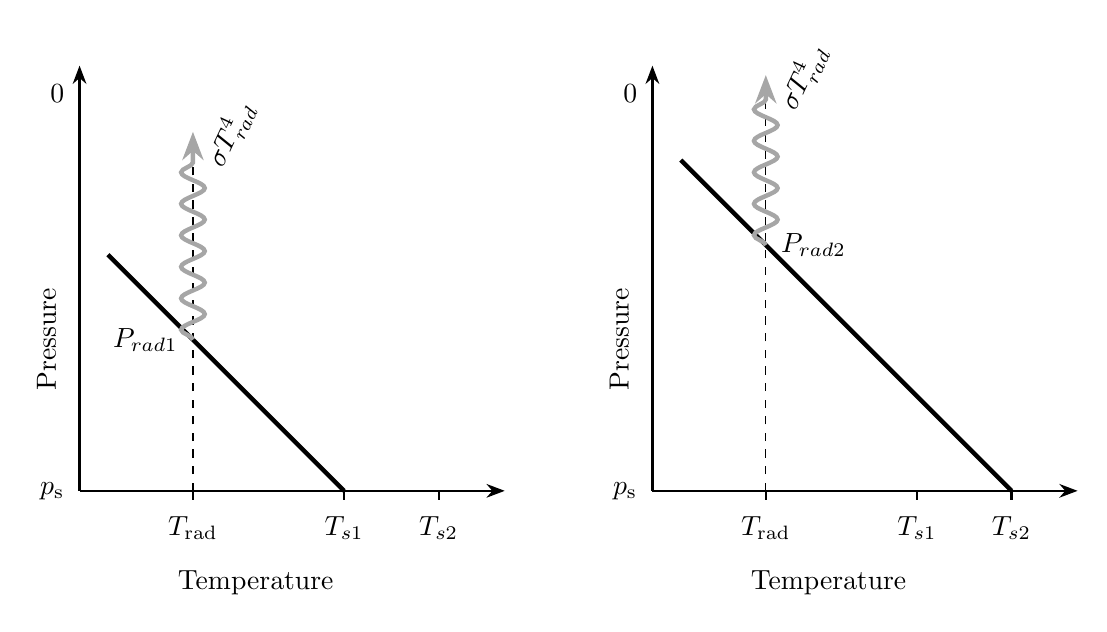
\begin{tikzpicture}[
    scale=1.2,
    >=Stealth,
    axis/.style={->, thick},
    line/.style={ultra thick},
    dashed line/.style={dashed, thin},
    wavy arrow/.style={
        gray!70,
        ultra thick,
        ->,
        decorate,
        decoration={snake, amplitude=1.5mm, segment length=4mm, post length=3mm}
    }
]

% ==================== LEFT SUBPLOT ====================
\begin{scope}[xshift=0cm]
    % Axes
    \draw[axis] (0,0) -- (4.5,0) node[below=25pt, xshift=-90pt] {Temperature};
    \draw[axis] (0,0) -- (0,4.5);

    % Axis Labels
    \node[left=2pt] at (0,0) {$p_{\text{s}}$};
    \node[left=2pt] at (0,4.2) {$0$};
    \node[left=12pt, rotate=90] at (0,2.25) {Pressure};

    % Ticks on X-axis
    \draw[thick] (1.2,0) -- (1.2,-0.1) node[below=2pt] {$T_{\text{rad}}$};
    \draw[thick] (2.8,0) -- (2.8,-0.1) node[below=2pt] {$T_{s1}$};
    \draw[thick] (3.8,0) -- (3.8,-0.1) node[below=2pt] {$T_{s2}$};

    % Temperature Line
    \draw[line] (0.3,2.5) -- (2.8,0);

    % Point Prad1
    \coordinate (P1) at (1.2,1.6);
    \node[left=2pt] at (P1) {$P_{rad1}$};

    % Dashed vertical line down to axis
    \draw[dashed line] (1.2,0) -- (1.2,3.8);

    % Wavy Arrow
    \draw[wavy arrow] (1.2,1.6) -- (1.2,3.8);

    % Radiation Label
    \node[above right=15pt, rotate=65] at (1.2,2.8) {$\sigma T_{rad}^4$};
\end{scope}

% ==================== RIGHT SUBPLOT ====================
\begin{scope}[xshift=0.5\textwidth]
    % Axes
    \draw[axis] (0,0) -- (4.5,0) node[below=25pt, xshift=-90pt] {Temperature};
    \draw[axis] (0,0) -- (0,4.5);

    % Axis Labels
    \node[left=2pt] at (0,0) {$p_{\text{s}}$};
    \node[left=2pt] at (0,4.2) {$0$};
    \node[left=12pt, rotate=90] at (0,2.25) {Pressure};

    % Ticks on X-axis
    \draw[thick] (1.2,0) -- (1.2,-0.1) node[below=2pt] {$T_{\text{rad}}$};
    \draw[thick] (2.8,0) -- (2.8,-0.1) node[below=2pt] {$T_{s1}$};
    \draw[thick] (3.8,0) -- (3.8,-0.1) node[below=2pt] {$T_{s2}$};

    % Temperature Line (Extended upwards to simulate higher pressure / greenhouse effect)
    \draw[line] (0.3,3.5) -- (3.8,0);

    % Point Prad2
    \coordinate (P2) at (1.2,2.6);
    \node[right=2pt] at (P2) {$P_{rad2}$};

    % Dashed vertical line down to axis
    \draw[dashed line] (1.2,0) -- (1.2,4.3);

    % Wavy Arrow
    \draw[wavy arrow] (1.2,2.6) -- (1.2,4.4);

    % Radiation Label
    \node[above right=15pt, rotate=65] at (1.2,3.4) {$\sigma T_{rad}^4$};
\end{scope}

\end{tikzpicture}

}
\end{figure}


Si l'atmosphère est optiquement épaisse, nous pouvons la découper en un empilement de tranches d'épaisseur $\Delta p_1$ telles que $\kappa q \Delta p_1/g = 1$. Chacune de ces tranches rayonne comme un corps noir idéal avec une température approximativement égale à la température moyenne de la tranche. Rappelons, cependant, qu'une autre propriété fondamentale des corps noirs est qu'ils sont des absorbeurs parfaits (bien que, s'ils ne sont des corps noirs que dans l'infrarouge, ils ne seront des absorbeurs parfaits que dans l'infrarouge). Par conséquent, le rayonnement infrarouge ne s'échappe vers l'espace qu'à partir de la tranche la plus élevée. L'OLR sera déterminé par la température de cette seule tranche, et sera insensible à la température des parties inférieures de l'atmosphère. La pression à la base de la tranche la plus élevée est $\Delta p_1$. Nous pouvons ainsi identifier $\Delta p_1$ comme le niveau de pression caractéristique à partir duquel le rayonnement s'échappe vers l'espace, qui sera par conséquent appelé $p_{rad}$ dans les discussions ultérieures. Le rayonnement s'échappant vers l'espace – l'OLR – sera alors d'environ $\sigma T(p_{rad})^4$.
Puisque la température diminue avec l'altitude sur l'adiabatique, l'OLR est inférieur à $\sigma T_s^4$ dans la mesure où $p_{rad} < p_s$. Comme le montre la Fig. 3.6, un gaz à effet de serre agit comme une couverture isolante, réduisant le taux de perte d'énergie vers l'espace pour n'importe quelle température de surface donnée. Toutes choses égales par ailleurs, la température de surface à l'équilibre d'une planète ayant un gaz à effet de serre dans son atmosphère doit être supérieure à celle d'une planète sans gaz à effet de serre, afin de dissiper l'énergie par rayonnement à un rythme suffisant pour équilibrer le rayonnement solaire absorbé. L'enseignement clé à tirer de cette discussion est que l'effet de serre ne fonctionne que dans la mesure où l'atmosphère est plus froide au niveau de rayonnement qu'elle ne l'est au sol.
\end{document}
